
\chapter{Laufzeitsicht}

\section{Sequenzdiagramme}
\textbf{Szenario I: Auswählen eines Roboters}\\

\begin{figure}[h]
    \centering
    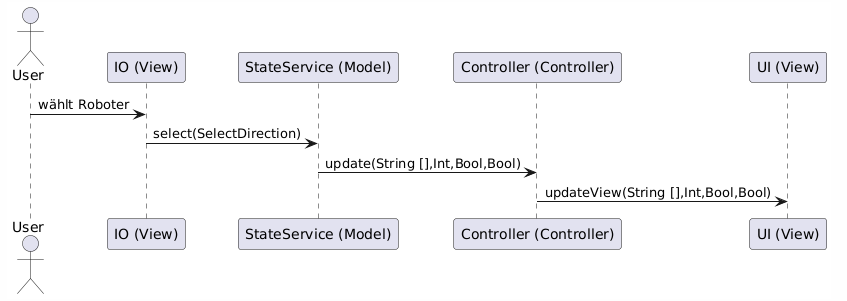
\includegraphics[width=0.8\linewidth]{diagrams/selectBefehl250625.png}
    \caption{Auswahl des Roboters}
    \label{fig:Auswahl}
\end{figure}

\clearpage\textbf{Szenario II: Bewegungsbefehl über GUI}\\

\begin{figure}[h]  
    \centering
    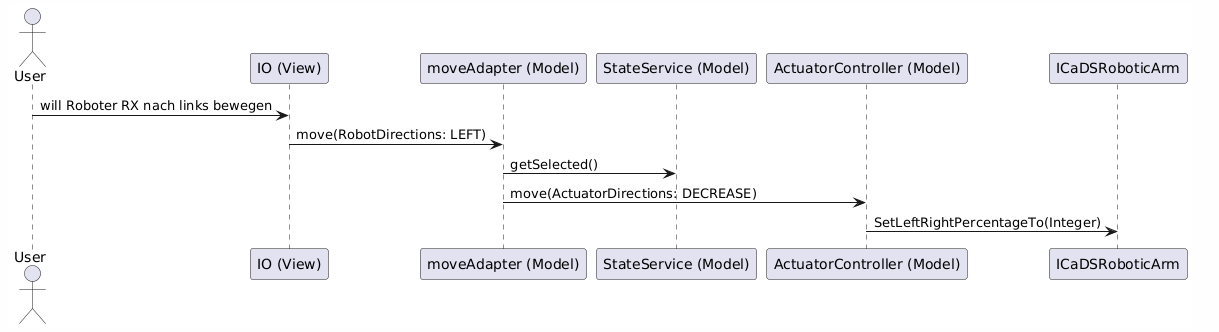
\includegraphics[width=0.8\linewidth]{diagrams/moveBefehl250625.png}
    \caption{Bewegungsbefehl über GUI}
    \label{fig:Bewegungsbefehl}
\end{figure}

\textbf{Szenario III: Watchdog}\\
\begin{figure}[h]  
    \centering
    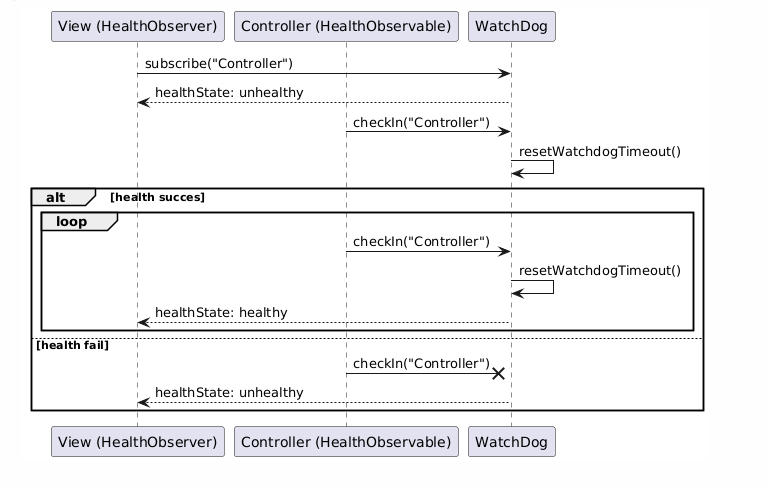
\includegraphics[width=0.8\linewidth]{diagrams/watchdog260625.png}
    \caption{Watchdog}
    \label{fig:Watchdog}
\end{figure}


\clearpage
\section{FSM-Diagramme}

\textbf{FSM I: UI}\\
\begin{figure}[h]  
    \centering
    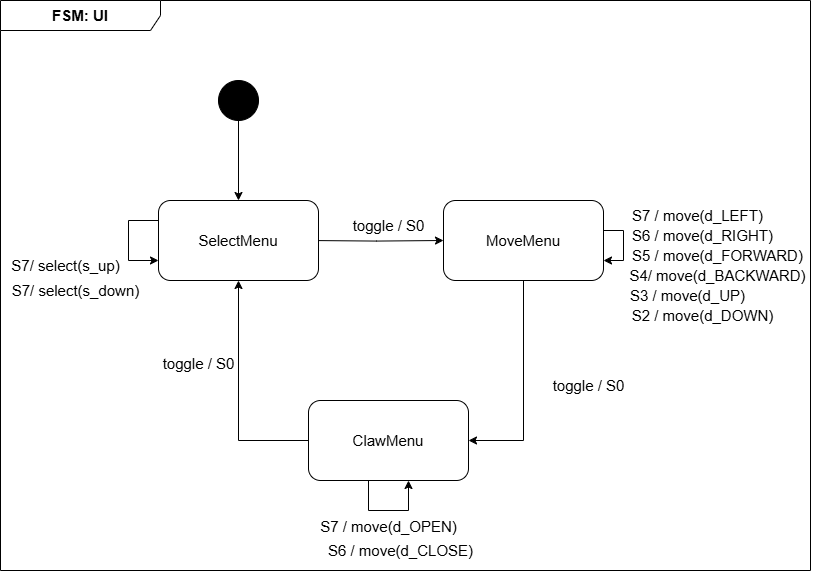
\includegraphics[width=0.8\linewidth]{diagrams/FSM_UI.drawio.png}
    \caption{UI States Diagramm}
    \label{fig:UI_States_Diagramm}
\end{figure}

\clearpage 
\section{Aktivitätsdiagramme}





%\section{Szenario III}
%\textbf{Fehlerfall: Verbindung zu Roboter fällt aus}\\

%\begin{figure}[h]  
%    \centering
%    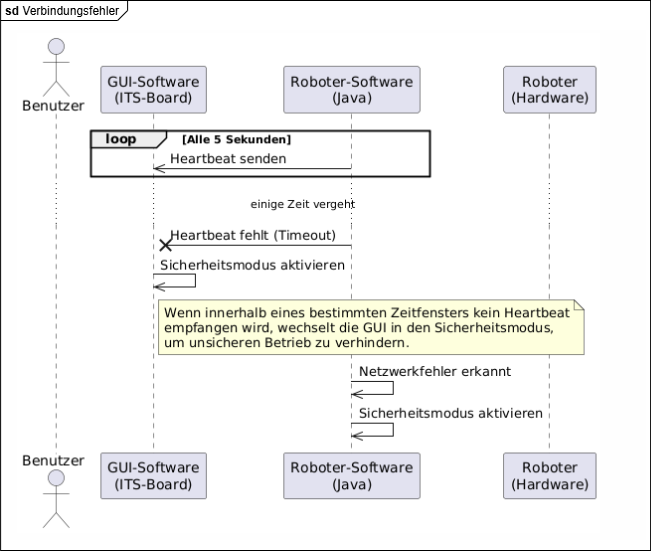
\includegraphics[width=0.8\linewidth]{diagrams/Verbindungsverlust.png}
%    \caption{Verbindungsverlust}
%    \label{fig:Verbindungsverlust}
%\end{figure}



